\subsection{Quality of Service}

There are different ways to approach implementing a DDS. When a DDS is referred to as a data-centric \emph{middleware}, it means that the systems infrastructure takes more responsibility to reach its goal.

The fundamental goal is to get the right data, to the right place, at the right time.

In order to ensure a level of quality depending on the requirements, a Quality of Service exist to reach the goal.

Figure \ref{DeInPa} contains an overview of different parameters that can be configured to meet the requirement depending on the need.

\begin{figure}[h]
\centering
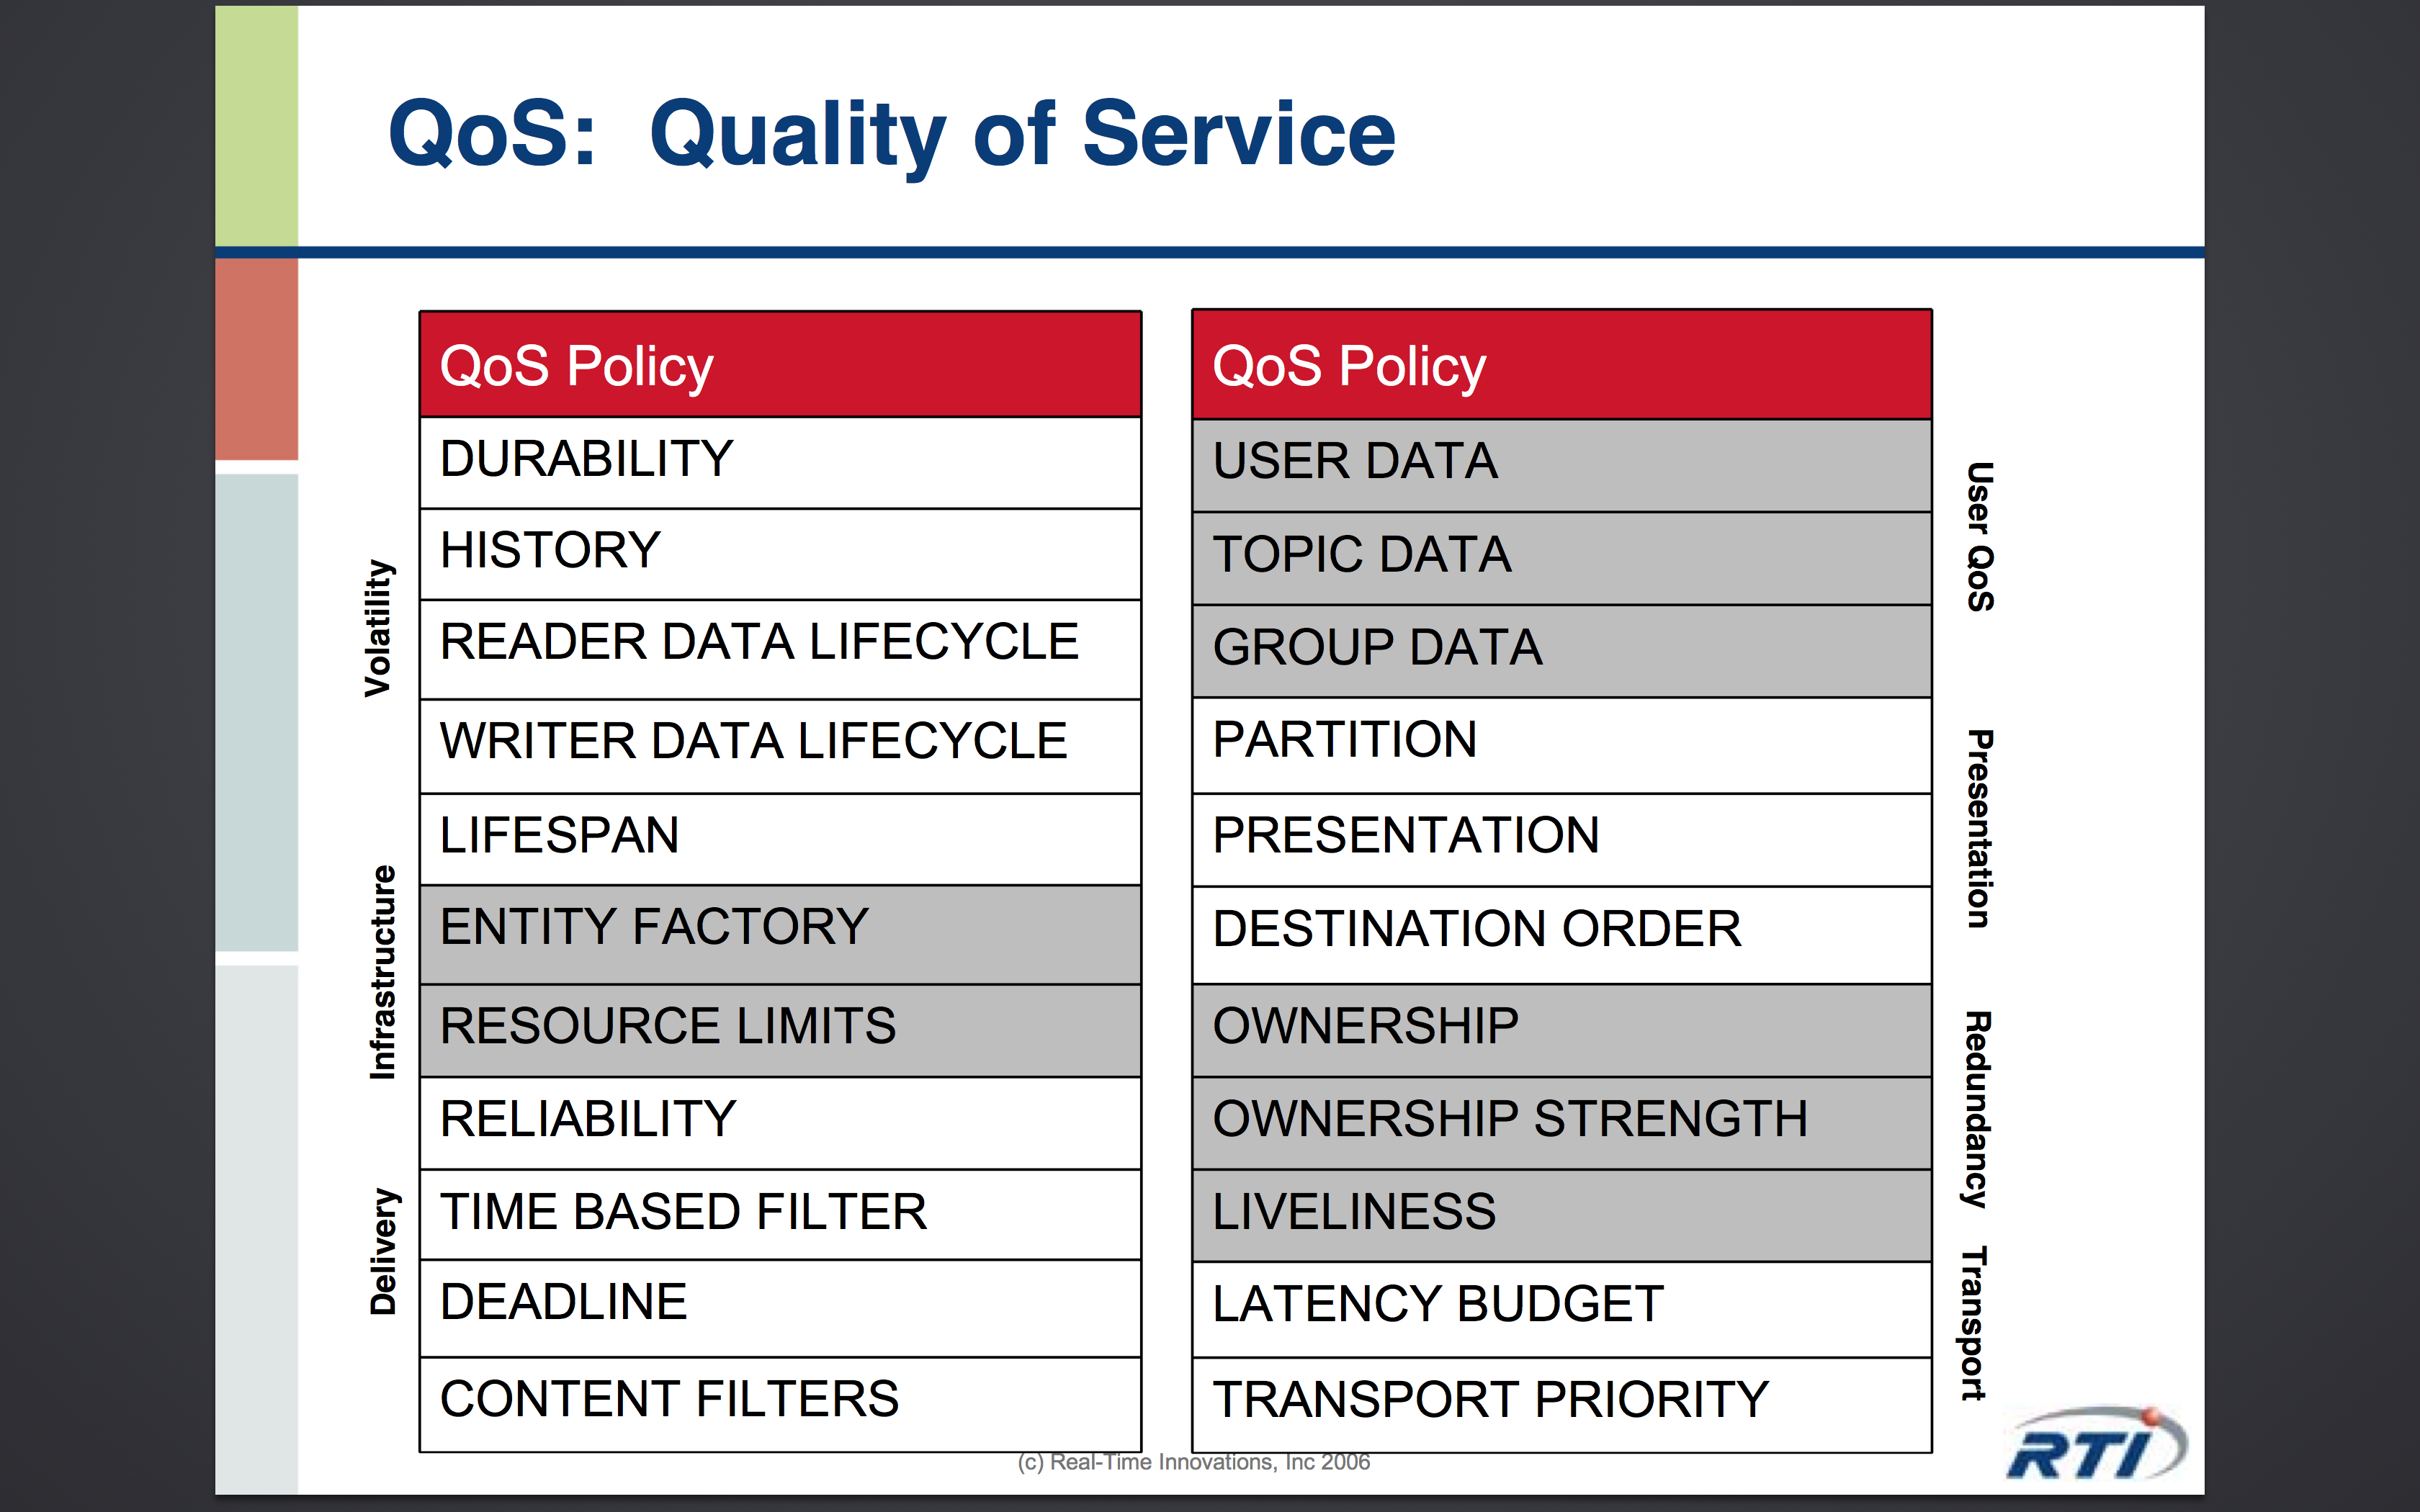
\includegraphics[height=100mm, keepaspectratio]{img/dds_question_4-6/QoS_services}
\caption{QoS - Services}
\label{QoS - Services}
\end{figure}

\newpage

With these parameters a node or topic can be configured to meet certain requirements.

An example where we have the following requirements:

\begin{itemize}
\item Single dataWriter, but multiple dataReaders
\item For every new dataReader that joins the topic should get the last set of data
\item Every dataReader should get all issued data
\end{itemize}

To ensure the requirement will be met, we can achieve it by making use of the services provided by the QoS. The requirement could be met by using the following services:

\begin{itemize}
\item History (Keep Last)
\begin{itemize}
\item To control how much data needs to be available
\end{itemize}
\item Reliability
\begin{itemize}
\item To ensure that data is delivered
\end{itemize}
\item Lifespan
\begin{itemize}
\item To know how and where data is stored
\end{itemize}
\end{itemize}